\documentclass[12pt]{amsart}

%Below are some necessary packages for your course.
\usepackage{amsfonts,latexsym,amsthm,amssymb,amsmath,amscd,euscript,tikz}
\usepackage{framed}
\usepackage{fullpage}
\usepackage{comment}
\usepackage{tikz}
\usepackage{bm}
\usepackage{enumerate}
\usepackage{dsfont}
\usepackage{hyperref}
\usetikzlibrary{patterns}
\usepackage{subfig}
\usepackage{float}
\usepackage{listings}
% \usepackage[cache=false]{minted}

\lstset{
  basicstyle=\footnotesize,
  xleftmargin=.2\textwidth, xrightmargin=.2\textwidth
}

\usetikzlibrary{decorations.markings,decorations.pathmorphing}
\usepackage{tikz-cd}
\usepackage{enumitem}
\usepackage{hyperref}
    \hypersetup{colorlinks=true,citecolor=blue,urlcolor =blue,linkbordercolor={1 0 0}}

\newenvironment{statement}[1]{\smallskip\noindent\color[rgb]{0.0,0.0,0.0} {\bf #1.}}{}
\newenvironment{solution}[1]{\vspace{5mm}\smallskip\noindent\color[rgb]{0.0,0.0,0.75} {\bf #1.}}{}
\allowdisplaybreaks[1]

%Below are the theorem, definition, example, lemma, etc. body types.

\newtheorem{theorem}{Theorem}
\newtheorem*{proposition}{Proposition}
\newtheorem{lemma}[theorem]{Lemma}
\newtheorem{corollary}[theorem]{Corollary}
\newtheorem{conjecture}[theorem]{Conjecture}
\newtheorem{postulate}[theorem]{Postulate}
\theoremstyle{definition}
\newtheorem{defn}[theorem]{Definition}
\newtheorem{example}[theorem]{Example}

\theoremstyle{remark}
\newtheorem*{remark}{Remark}
\newtheorem*{notation}{Notation}
\newtheorem*{note}{Note}

% You can define new commands to make your life easier.
\newcommand{\BR}{\mathbb R}
\newcommand{\BC}{\mathbb C}
\newcommand{\BF}{\mathbb F}
\newcommand{\BQ}{\mathbb Q}
\newcommand{\BZ}{\mathbb Z}
\newcommand{\BN}{\mathbb N}
\newcommand{\BE}{\mathbb E}

\newcommand{\CU}{\mathcal{U}}
\newcommand{\CO}{\mathcal{O}}
\newcommand{\CC}{\mathcal{C}}
\newcommand{\Ob}{\operatorname{Ob}}
\newcommand{\Mor}{\operatorname{Mor}}


% We can even define a new command for \newcommand!
\newcommand{\C}{\mathbb{C}}
\newcommand{\F}{\mathbb{F}}
\newcommand{\Q}{\mathbb{Q}}
\newcommand{\Z}{\mathbb{Z}}
\newcommand{\R}{\mathbb{R}}
\newcommand{\N}{\mathbb{N}}
\newcommand{\bP}{\mathbb{P}}

\newcommand{\Hom}{\operatorname{Hom}}
\newcommand{\End}{\operatorname{End}}
\newcommand{\ch}{\operatorname{char}}
\newcommand{\image}{\operatorname{im}}
\newcommand{\kernel}{\operatorname{ker}}
\newcommand{\rank}{\operatorname{rank}}
\newcommand{\sym}{\operatorname{Sym}}
\newcommand{\im}{\operatorname{im}}
\newcommand{\lcm}{\operatorname{lcm}}
\newcommand{\Res}{\operatorname{Res}}

\newcommand{\Pois}{\text{Pois}}
\newcommand{\ex}{\text{exp}}
\newcommand{\Var}{\text{Var}}
\newcommand{\Binom}{\text{Binom}}
\newcommand{\btheta}{\bm\theta}
\newcommand{\bT}{\bm T}
\newcommand{\E}{\mathbb{E}}
\newcommand{\I}{\mathbb{I}}
\newcommand{\BP}{\mathbb{P}}
\newcommand{\x}{\bm x}
\newcommand{\y}{\bm y}
\newcommand{\z}{\bm z}
\newcommand{\bmT}{\bm T}
\newcommand{\bmX}{\bm X}
\newcommand{\bmY}{\bm Y}
\newcommand{\bmZ}{\bm Z}
\newcommand{\br}{\bm r}
\newcommand{\bI}{\bm I}
\newcommand{\1}{\mathds{1}}



% If you want a new function, use operatorname to define that function (don't use \text)

\renewcommand{\baselinestretch}{1.25}
\usepackage{hyperref}

\hypersetup{
    colorlinks=true,
    linkcolor=teal,
    filecolor=teal,      
    urlcolor=teal
    }

\title{CS 182 Fall 2022, Problem Set 0}

\begin{document}

\maketitle

\vspace*{-0.25in}
\centerline{Due: September 12, 2022 11:59pm}

\begin{center}
\end{center}
\vspace*{0.15in}


\noindent This problem set is a review of concepts in probability and algorithms. Topics include conditional probability, Bayes rule, union bound, linearity of expectation, big O notation, and Python programming (algorithms, recursion, OOP).
\vspace*{0.35in}

\begin{statement}{1}
\textit{Probability.} (20 points) From all his years running the chocolate factory, Charlie knows that classic chocolate bars that crack before reaching store shelves have a 2 in 300 chance of having air bubbles on the surface. He also knows that surface bubbles appear on 1 in 50 classic bars that won't crack as well. Looking through his files, Charlie's most recent Food Standards Agency report states that 1 in 100 classic bars from his factory crack before reaching the shelves.

\begin{enumerate}
    \item (5 points) Charlie just produced a test bar using his classic chocolate bar recipe, and it comes out with surface bubbles. Assuming that Charlie decides to ship and sell this bar, what is the probability that the bar cracks before reaching store shelves?
    \\ Let $B$ be the event that a chocolate bar has air bubbles on the surface and let $C$ be the event that a chocolate bar cracks before reaching the store. Then we are 
    interested in the quantity 
    $$
        \Pr{[C|B]} = \frac{\Pr{[B|C]}\Pr{[C]}}{\Pr{[B}]}
    $$
    where the right-hand side is true by Bayes rule. Then, 
    \begin{align*}
        \Pr{[B]} &= \Pr{[B|C]}\Pr{[C]} + \Pr{[B|C']}\Pr{[C']} \\ 
        &= \frac{2}{300}*\frac{1}{100} + \frac{1}{50}*\frac{49}{50}\\ 
        &= \frac{59}{3000}
    \end{align*}
    Then, 
    \begin{align*}
        \Pr{[C|B]} &= \frac{\Pr{[B|C]}\Pr{[C]}}{\Pr{[B}]} \\
        &= \frac{\frac{1}{50}* \frac{49}{50}}{\frac{59}{3000}} \\ 
        &= \frac{294}{295}
    \end{align*}

    \item (5 points) Charlie's factory makes 10,000 classic chocolate bars: 4,470 come out with surface bubbles and the rest do not. What is the expected number of cracked bars in this batch?
    \\Given that we know how many bars have bubbles and how many do not, we can calculate the expected number of cracked bars as a sum of 
    the expected number of bars with bubbles that will crack and the expected number of bars without bubbles that will crack. Any given bar with bubbles has a 
    $\frac{2}{590}$ chance of cracking and all the bars crack independently of each other, so the number of bars with bubbles that will crack is distributed binomial, which 
    has expectation 
    $$
        p*n
    $$
    where $p$ is the probability that a bar will crack (the conditional probability) and the $n$ is the number of bars in question. So we first find 
    \begin{align*}
        \Pr{[C|B']} &= \frac{\Pr{[B'|C]}\Pr{[C]}}{\Pr{[B']}} \\ 
        &= \frac{(1 - \frac{2}{300}) * \frac{1}{100}}{1 - \frac{59}{300}} \\ 
        &= \frac{149}{14705}
    \end{align*}
    Thus, the expected number of bars that will crack in this batch is 
    $$
        4470*\frac{2}{590} + 5530*\frac{149}{14705} \approx 71.186
    $$

    \item (10 points) There was a mistake at the chocolate factory and peanuts were accidentally added to the liquid chocolate being used to create plain chocolate bars. Luckily, not that many peanuts were added so the probability of each chocolate bar produced in the next hour (until this batch of liquid chocolate is used up) having any peanuts in it is distributed \textit{IID}\footnote{In practice, the occurrence of peanuts in chocolate bars under this setting may not be IID since there may be parts of the liquid chocolate where peanuts are more concentrated than others e.g. if peanuts are more dense than chocolate, they would tend to fall to the bottom of the chocolate vat or if less dense, would tend to float to the surface.} with the probability of containing peanuts being $1/2$ for each bar. 
    
    \noindent If we examine chocolate bars until we find one with peanuts, is the expected number of regular plain bars observed more than the expected number of peanut bars observed within the batch of total bars examined? What if our stopping condition changes to seeing a total of 2 bars with added peanuts, how would your previous answer change (if at all)? Explain your reasoning and show your work.
    
    \noindent\textbf{Hint}: Denoting the random variable of interest by $X$, define a suitable event, $A$, and use the law of total expectation: $\E[X] = \E[X|A]\Pr[A] + \E\left[X|\,\overline{A}\,\right]\Pr\left[\,\overline{A}\,\right]$.
    \\ 
    Let $X$ be the number of plain bars observed before observing a bar with peanuts in it and let $Y$ be the number of plain 
    bars observeed before observing 2 peanuts bars. Further, let $A$ be the event that the first bar that is inspected has peanuts in it.
    Then, 
    \begin{align*}
        \E[X] &= \E[X|A]\Pr[A] + \E\left[X|\,\overline{A}\,\right]\Pr[\,\overline{A}]\\ 
        &= 0*\frac{1}{2} + (1 + \E[X])*\frac{1}{2}\\ 
        &\Downarrow\\ 
        \E[X] &= 1
    \end{align*}
    $E[X|A] = 0$ because if the first bar that was observed had peanuts then our stopping condition is met, so we observed 
    0 plain bars. $E[X|\overline{A}] = 1 + E[X]$ because if the first bar we observed was a plain bar, then we add it to the total 
    number of plain bars we have seen and are back at the starting point i.e. how many plain bars do we observe before we observe a peanut 
    bar. $\Pr[A] = \Pr[\overline{A}] = 1/2$ by the problem description. Also, the expected number of peanut bars seen is always one because 
    we stop exactly when we see one peanut bar. Hence, the expected number of plain bars observed is equal to the expected number of peanut bars 
    observed when we examine bars until we see a peanut bar. \\When the stopping condition is 2 peanut bars, we have 
    \begin{align*}
        \E[Y] &= \E[Y|A]\Pr[A] + \E[Y|\overline{A}]\Pr[\overline{A}]\\
        &= \E[X]*\frac{1}{2} + (1 + \E[Y])\frac{1}{2} \\ 
        &= \frac{1}{2} + \frac{1}{2} + \frac{\E[Y]}{2} \\ 
        &\Downarrow\\ 
        \E[Y] &= 2
    \end{align*}
    $\E[Y|A] = \E[X]$ because if the first bar we observe is a peanut bar, then we stop examining bars after seeing another peanut bar i.e. we 
    stop examining bars after seeing one peanut bar, which is $\E[X]$. $\E[Y|\overline{A}] = 1 + \E[Y]$ because if the first bar 
    we observed was a plain bar then we are back at square one. Like before, the expected number of peanut bars seen is trivially 2; hence, 
    even when the stopping condition is 2 peanut bars, the expected number of plain bars observed is equal to the expected number of peanut bars 
    observed. 
\end{enumerate}
\end{statement}


\newpage
\begin{statement}{2}
\emph{Algorithms.} (20 points) Assume we are working with an array of $n$ floating point numbers that are sampled from the uniform distribution over the interval $[0,M]$. Consider the following sorting algorithm:
\begin{enumerate}
    \item Create $k = \Theta(n)$ empty arrays, e.g. $n/2$
    \item For each element $X$ in the input array of length $n$, insert $X$ into the array indexed at int($\frac{X}{M}*k$), where the int() operator performs truncation and the arrays are indexed starting at 0. 
    \item Sort each of these $k$ arrays using insertion sort
    \item Create an output sorted array by concatenating each of the $k$ arrays in order to arrive at the overall sorted output array of numbers
\end{enumerate}
Show that the average-case runtime\,---\,i.e., the expectation, over the randomly sampled elements\,---\,of the algorithm used in this setting is $O(n)$. 

\noindent\textbf{Hint:} Reason about each step separately; the challenge is to analyze Step (3). For that, note that if array $i$ contains $n_i$ elements, the running time of insertion sort is $O((n_i)^2)$. But what is $n_i$, given the assumption of uniformly distributed elements? Use a Bernoulli random variable $X_{ij}$ to model the inclusion of the $j$th element of the input array in the $i$th array for each element. You may find the following equality helpful given that $n_i = \sum_{j=1}^nX_{ij}$: $$\mathbb{E}\left[n_i^2\right] = \mathbb{E}\left[ \sum_{j=1}^{n}X_{ij}^2 \right] + \mathbb{E}\left[\sum_{j=1}^n\sum_{k\neq j} X_{ij}X_{ik} \right].$$
\begin{enumerate}
    \item This first step can be accomplished in $O(n)$ time
    \item Assuming truncation, division, multiplication, and indexing can be done in constant time, step two can also be completed in $O(n)$ time because we have to iterate 
    through each of the $n$ floating point numbers to complete the computations. 
    \item First, let $n_i$ be the number of elements in one of the $k$ arrays. Also, let $X_{ij}$ be the indicator random variable that is 
    1 if floating point number ${j}$ is included in array $i$. Therefore, 
    $$
        n_i = \sum_{j=1}^n X_{ij}
    $$
    We sort $k$ arrays using insertion sort, so the average expected runtime is 
    $$
        O\Big(\sum_{1}^k\E(n_i^2)\Big)
    $$
    Handling the expectation first, we see that
    \begin{align*}
        \E(n_i^2) &= \E\Big(\sum_{j=1}^nX_{ij} \sum_{k=1}^nX_{ik} \Big)\\
        &= \E\Big(\sum_{j=1}^n\sum_{k=1}^nX_{ij}X_{ik}\Big)\\ 
        &= \E\Big( \sum_{j=1}^n X_{ij}^2 + \sum_{j=1}^n\sum_{j\neq k} X_{ij}X_{ik} \Big)\\ 
        &= \E\Big(  \sum_{j=1}^n X_{ij}^2 \Big) + \E\Big( \sum_{j=1}^n\sum_{j\neq k} X_{ij}X_{ik} \Big)\\ 
        &= \sum_{j=1}^n\E(X_{ij}^2) + \sum_{j=1}^n\sum_{j\neq k}E(X_{ij}X_{ik})
    \end{align*}
    The third to last line is true if we separate the cases where $j=k$ and $j\neq k$. Then we have $\E(X_{ij}^2) = \E(X_{ij}) = \frac{1}{k}$ because 
    each number is included in an array with probability $\frac{1}{k}$. This also holds true for each of the indicator variables on the right side 
    of the equality, so $\E(X_{ij}X_{ik}) = \frac{1}{k^2}$. Thus, 
    \begin{align*}
        \E(n_i^2) &= \sum_{j=1}^n\E(X_{ij}^2) + \sum_{j=1}^n\sum_{j\neq k}E(X_{ij}X_{ik})\\ 
        &= \sum_{j=1}^n\frac{1}{k}  + \sum_{j=1}^n\sum_{j\neq k}\frac{1}{k^2}\\ 
        &= \frac{n}{k} + \frac{n(n-1)}{k^2}\\ 
        &= \frac{kn + n^2 - n}{k^2}
    \end{align*}
    Returning to the runtime calculation, we now substitute to find the following
    \begin{align*}
        O\Big(\sum_{1}^k \E(n_i^2)\Big) &= O\Big(\sum_1^k \frac{kn + n^2 - n}{k^2}\Big)\\ 
        &= O\Big(\frac{kn + n^2 - n}{k}\Big)\\ 
        &= O\Big( \frac{n^2}{k} + n - \frac{n}{k} \Big)
    \end{align*}
    \item The last step requires $O(k)$ time. 
    \item Putting everything together, we have that the total time complexity is the following:
    \begin{align*}
        O(n) + O(n) + O\Big( \frac{n^2}{k} + n - \frac{n}{k} \Big) + O(k) &= O\Big( \frac{n^2}{k} + n - \frac{n}{k} + k \Big)
    \end{align*}
    Finally, we use that $k = \Theta(n)$ to simplify the right hand side of the equality:
    \begin{align*}
        O\Big( \frac{n^2}{k} + n - \frac{n}{k} + k \Big) &= O\Big( n + n - 1 + n \Big)\\ 
        &= O(n)
    \end{align*}

\end{enumerate}
\end{statement}


\newpage
\begin{statement}{3}
\emph{Programming Warm-Up.} (20 points)  
\begin{enumerate}
    \item \emph{Pascal's Triangle.} (10 points)
            \newline Write an iterative algorithm to generate the $0$th to $n$th rows of Pascal's triangle where indexing starts at 0. E.g. the triangle corresponding to $n=5$ will have 6 rows in total, one for the 0th row, the 1st row, etc. up until the 5th row. Complete the function in the \texttt{pset0.py} file and test your function against the provided test cases to make sure that it is working. Do not use any external libraries or online solutions, please use only base python functions and data types.
            
            \noindent More info about Pascal's Triangle can be found \href{https://en.wikipedia.org/wiki/Pascal\%27s\_triangle}{here}. \newline
            
    \item \emph{Flatten Nested Lists.} (10 points)
            \newline Write a recursive algorithm that outputs a list of integers which are extracted from a nested set of iterable lists. Your function should flatten a nested structure of integers contained in various lists into a simple list of integers. For example if the input is [1,2,[3,4],[[5],6,7]] then return [1,2,3,4,5,6,7].
           
           \noindent Please be sure to use recursion for this exercise. Complete the function in the \texttt{pset0.py} file and test your function against the provided test cases to make sure that it is working. Do not use any external libraries or online solutions, please use only base python functions and data types.
\end{enumerate}
\end{statement}

\newpage
\begin{statement}{4}
\emph{Encryption Algorithms.} (35 points)
\begin{enumerate}
    \item \textit{Caesar Cipher.} (10 points)
        \begin{enumerate}
            \item (8 points) Complete the class declaration in \texttt{pset0.py} to create a custom, user-defined data structure that can save a cipherkey, an alphabet, and also perform encryption and decryption of a message using a Caesar Cipher. A Caesar Cipher is a simple encryption method that shifts all letters by a fixed offset specified by the cipherkey's location in the alphabet. E.g. if our alphabet is the standard lower-case English letters abc...xyz and our message is ``x" and our cipherkey is ``b" then the resulting ciphertext would be ``y" since the cipherkey ``b" corresponds to the index 1 letter of the alphabet so we offset the plaintext message ``x" by +1 letter to get ``y". If our cipherkey was ``d", we would offset by 3 since ``d" is at index 3 in the alphabet (indexing from 0) which would result in our message being encrypted to ``a". We wrap around to the start of the alphabet if our offset exceeds the last letter. Likewise, for decryption, instead of offsetting forward, we offset backwards to decrypt a ciphertext into plaintext. The diagram below illustrates how a Caesar cipher as described above would decrypt ciphertext to readable plaintext for a cipherkey of ``d" corresponding to a 3 letter shift.
        
        
        \begin{figure}[H]
            \centering
            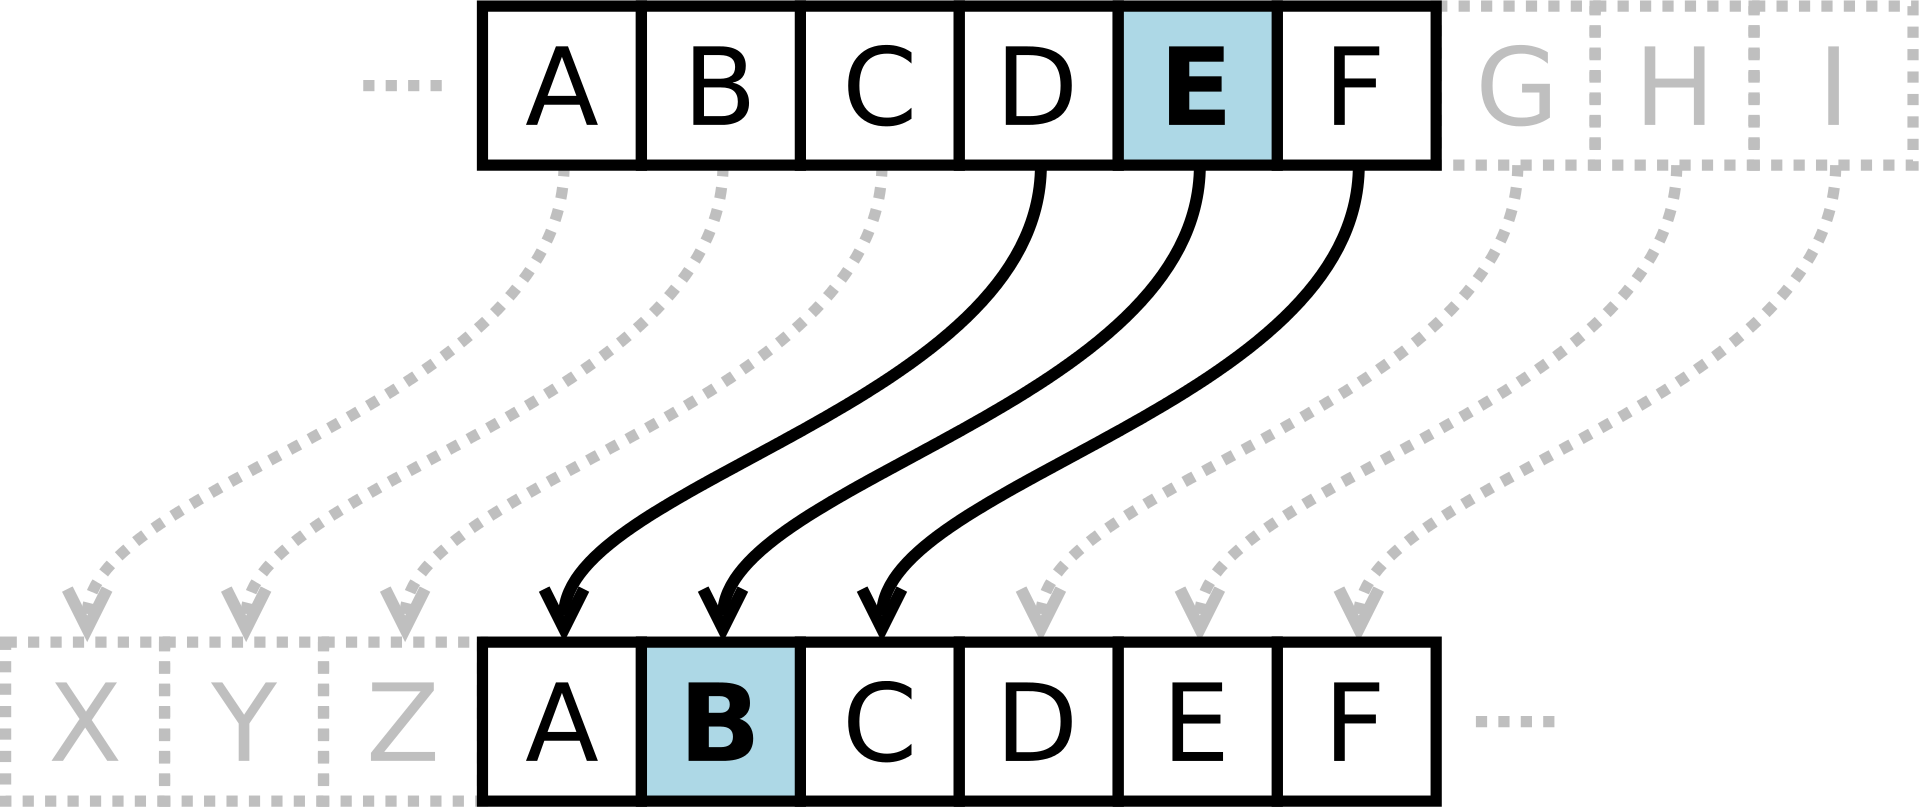
\includegraphics[width=0.7\textwidth]{images/caesar_cipher.png}
            \caption{Source:  \href{https://en.wikipedia.org/wiki/Caesar\_cipher}{https://en.wikipedia.org/wiki/Caesar\_cipher}}
        \end{figure}
        
            \item (2 points) Bob thinks he's clever by encrypting his secret message not once, but twice using cipherkeys ``h" and ``t" respectively. What is the issue with Bob's approach? Would it make a difference if he reversed the order of the cipherkeys applied? (i.e. ``t" then ``h") \footnote{\textit{Note:} In-depth knowledge of ciphers is not required to answer the logical reasoning questions in this section, just critical thinking. Short answers are fine, you can answer with just a sentence or two.}
            7 19 
            \\The issue with Bob's approach is that encrypting by "h" (index 7) and then "t" (index 19) is the same as encrypting with 
            "z" (index = 7 + 19  = 26). If we let a=0, b=2,...,z=26 and denote the index of a character to be encrypted as $n$, then the encryption function 
            $E$ with cipher key $c$ works as 
            $$
                E(n) = (n + c) \mod 26
            $$
            So, first encrypting with $h$ gives $E(n) = (n + h) \mod 26$, and then encrypting that with $t$ gives $E(E(n)) = (n + h) + t = n + (h + t) \mod 26$. This proves the claim above 
            and also shows that reversing the cipherkeys does not make a difference because $(h + t) = (t + h) \mod 26$. 
        \end{enumerate}
        
    \newpage
    \item \textit{Caesar Cipher Auto-Decryption.} (10 points)
        \begin{enumerate}
            \item (10 points) Add to the \texttt{CaesarCipher} class a new method called \texttt{auto\_decrypt()} that will automatically try to guess the correct cipherkey of the message by trying each character in the saved alphabet and computing the \% of words recognized in the English language contained in the resulting plaintext. Return a tuple containing the decrypted plaintext and  auto-detected cipherkey. You may add early stopping and stop if you find a cipherkey that produces a plaintext output with  at least 85\% words recognized in the English word dictionary. If no key produces at least 85\% recognizable words, then return the key with the highest \% of recognized words. The \texttt{english\_word\_list} has been read in for you, pass in this object by reference into your method call. Add an optional argument called \texttt{verbose} with a default of False that will print out the percentage of words recognized as English words for each character tried as the cipherkey to track the progress of your auto-detection method.
            \item \textit{Bonus problem.} (5 bonus points) Can you think of a faster way to auto-decrypt a secret message (in English) that was encrypted using a Caesar cipher? Briefly describe your approach and add an additional method to \texttt{CaesarCipher} in \texttt{pset0.py} called \texttt{auto\_decrypt\_bonus()} if you're up for the challenge. The top 5 fastest submissions by average runtime on a set of hidden test cases that return the correct output for all test cases will earn extra credit on this assignment. The class object is instantiated once at the start and all test cases are run on it.
            
            \noindent\textbf{Hint:} A table containing the average frequency of use for each letter in the alphabet in written English text has also been provided that you can utilize in your approach. Source: \href{https://en.wikipedia.org/wiki/Letter\_frequency}{https://en.wikipedia.org/wiki/Letter\_frequency}.
            \\ Suppose we encrypted an english message using key $c$. This message should roughly follow the letter frequencies 
            that were provided, and this is increasingly more likely as the length of the message grows. Every letter is shifted by some fixed offset, so every letter 
            $e$ corresponds to some letter $e + c_i \mod 26$ where $c_i$ corresponds to the index of the key, $c$, in the alphabet. So if we find the frequencies of the letters in the encrypted message then 
            the letters that appear the most are most likely to have been the letter $e$ in the original plaintext (because $e$ is the most frequent letter). The algorithm uses this idea by first going down the list of frequencies in the cipher text and 
            treating each as an encypted letter $e$. It finds the corresponding offset and then uses that offset to decrypt each letter in the table of ciphertext frequencies, and for each 
            letter that is in the correct place compared to the table of known frequencies, it adds 1 to a counter of satisfied frequencies (named 'sat' in the python program). The algorithm 
            returns the key whose offest matched the highest number decrypted ciphertext frequencies to actual letter frequencies. 
        \end{enumerate}
      
    
    \item \textit{Vigen\`ere Cipher.} (15 points)
        \begin{enumerate}
            \item (13 points) Implement a class-based Vigenère Cipher by completing the code for \texttt{VigenereCipher} in \texttt{pset0.py}. Your data structure should have a method for encryption and decryption. A Vigenère cipher can be thought of as a generalization of a Caesar cipher. Vigenère ciphers convert plaintext to ciphertext using a cipherkey that may be of length 1 or greater where each subsequent character in the cipherkey specifies the alphabetical offset for each subsequent plaintext letter being encrypted. We visualize the possible alphabetical offests using the following table:
            
            \begin{figure}[H]
            \centering
                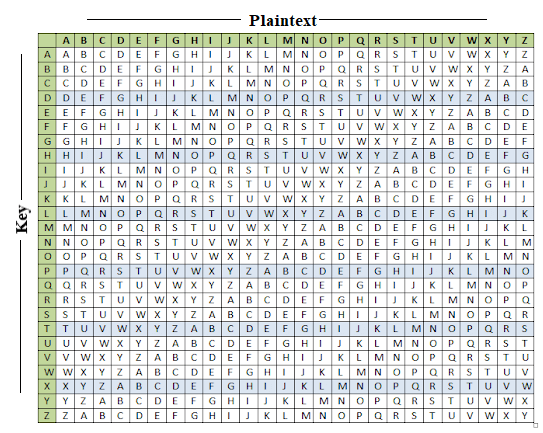
\includegraphics[width=.75\textwidth]{images/vigenere_cipher_table_hd.png}
                \caption{Source:  \href{https://i.ibb.co/GfDR26w/vigenere-cipher.png}{https://i.ibb.co/GfDR26w/vigenere-cipher.png}}
            \end{figure}
            The cipherkey is resued from start to end as many times as needed to encrypt or decrypt the entire message. A Caesar cipher is a special case of Vigenère Ciphers where the cipherkey is of length 1. 
            
            For example, consider the plaintext ``helloworld" and a cipherkey ``neat". We need to create a key with 10 characters, while neat only has 4. We therefore repeat our cipherkey to produce our final key: ``neatneatne". We then encrypt using the column for our first letter, ``h", using the row of our first letter of the cipher, ``n", to get the first letter of our ciphertext, ``t". Repeat the process to get the full ciphertext, ``tilebaokyg". We can then decrypt the first letter of our ciphertext, ``t", using the row of first letter of our cipherkey, "n", and locating the "t" in that row. ``t" in this row is located in column ``h", giving us our first plaintext letter. We repeat this process to then generate our full plaintext string ``helloworld". 
            
            \item (2 points) A Vernam cipher is a special case of a Vigenère cipher where the cipherkey must be at least as long as the plaintext input. Why might this be a stronger method of encryption then a regular Vigenère cipher? Assuming the cipherkey is a series of random characters, what would be the distribution of letters in the ciphertext would look like using this cipher?
            \\ If the letters in the cipherkey are completely random and each letter is individually encrypted, the distribution of letters in the cipher would appear completely random and no letter 
            would be any more or less significantly frequent than another. This prevents auto decryption methods, like the ones we saw in questions 2A and 2B, from deciphering the 
            cipher without the key because there wouldn't be any discernible patterns in the letters or words: this is why the Vernam Cipher is safer. 

        \end{enumerate}

\end{enumerate}
\end{statement}

\newpage
\begin{statement}{5}
\noindent \textbf{Collaboration, Calibration and References} (5 points).
\begin{enumerate}
    \item With whom did you work on this problem set? What (if any) references and/or resources did you use beyond the course lecture slides and textbook? 
    \\ No one.
    \item (5 points) Approximately how long did it take you to complete this problem set? Please complete this brief \href{https://forms.gle/4Mip65wtTpkNxBTj9}{survey} worth 5 points, graded for completion.\\
    4 hours. 
\end{enumerate}
\end{statement}

\end{document}